% !TEX root = ../main.tex

\chapter{负载侧：可变等离子体负载}
\label{chap:plasma}

\section{互感耦合回路}

实验四把 H 桥的负载由线性支路换成“原边线圈 + 副边等离子体回路”的耦合结构（图~\ref{fig:pl-model}）。原边从桥臂 A 出发，串入 $i\sub{cs}$ 测量和 20 $\mu\Omega$ 的电阻 $R\sub{cs}$，接到互感原边绕组后回到桥臂 B。副边经 $i\sub{p}$ 测量、可变电感 $L\sub{p}(t)$、可变电阻 $R\sub{p}(t)$ 构成回路。两支 100~k$\Omega$ 电阻分别并在 $L\sub{p}$ 和 $R\sub{p}$ 两端，只起数值作用。

\begin{figure}[htbp]
\centering
\begin{circuitikz}[font=\footnotesize, line width=0.55pt, >={Latex[length=1.5mm]}]
\ctikzset{bipoles/length=0.95cm, resistors/scale=0.75, inductors/scale=0.75, diodes/scale=0.75, sources/scale=0.8}
\newcommand{\qd}[4]{% x, y of collector, name, diode side
  \node[nigbt, anchor=C, scale=0.72] (#3) at (#1,#2) {};
  \draw (#3.E) -- ++(#4,0) coordinate (#3e) to[D*] ($(#3.C)+(#4,0)$) -- (#3.C);
}
\draw (-1.3,0) to[V, l=$U\sub{dc}$, invert] (-1.3,5) ;
\draw[line width=0.8pt] (-1.3,5) -- (9.4,5);
\draw[line width=0.8pt] (-1.3,0) -- (9.4,0);
\qd{0.6}{4.55}{Q1}{0.72}
\qd{0.6}{1.8}{Q2}{0.72}
\qd{9.4}{4.55}{Q3}{0.72}
\qd{9.4}{1.8}{Q4}{0.72}
\draw (0.6,5) -- (Q1.C);
\draw (Q1.E) -- (Q2.C) node[midway,circ] (A) {};
\draw (Q2.E) -- (0.6,0);
\draw (9.4,5) -- (Q3.C);
\draw (Q3.E) -- (Q4.C) node[midway,circ] (B) {};
\draw (Q4.E) -- (9.4,0);
\node[above left=0pt and 0pt of A, font=\footnotesize] {A};
\node[above right=0pt and 0pt of B, font=\footnotesize] {B};
\node[font=\scriptsize, text=inkmuted] at ($(Q1.G)+(-0.2,0)$) {$Q_1$};
\node[font=\scriptsize, text=inkmuted] at ($(Q2.G)+(-0.2,0)$) {$Q_2$};
\node[font=\scriptsize, text=inkmuted] at ($(Q3.G)+(-0.2,0)$) {$Q_3$};
\node[font=\scriptsize, text=inkmuted] at ($(Q4.G)+(-0.2,0)$) {$Q_4$};
\draw (A) to[short, i=$i\sub{cs}$] (1.95,0 |- A) to[R, l=$R\sub{cs}$] (3.1,0 |- A) -- (3.45,0 |- A) -- (3.45,3.55);
\coordinate (p1) at (3.45,3.55); \coordinate (p2) at (3.45,1.35);
\draw (p1) to[L, l_=$L_1$] (p2);
\draw (p2) -- (3.45,0.65) -- (8.75,0.65) -- (8.75,0 |- B) -- (B);
\coordinate (s1) at (4.35,3.55); \coordinate (s2) at (4.35,1.35);
\draw (s1) to[L, l=$L_2$] (s2);
\draw[<->, line width=0.45pt, color=inkmuted] (3.62,3.75) to[bend left=25] node[above, font=\scriptsize] {$k=0.99999$} (4.18,3.75);
\draw (s1) to[short, i=$i\sub{p}$] (5.25,3.55) to[vL, l=$L\sub{p}(t)$] (7.3,3.55) -- (7.75,3.55) to[vR, l=$R\sub{p}(t)$] (7.75,1.35) -- (s2);
\end{circuitikz}
\caption{H 桥与互感耦合可变负载的主电路（数值并联电阻和缓冲电阻未画出）}
\label{fig:pl-model}
\end{figure}

两绕组自感都是 1~H、耦合系数 $k=0.99999$，可以近似为理想变压器。励磁电流和磁链为
\begin{equation}
i\sub{m}=i\sub{cs}-i\sub{p},\qquad \psi=L_1i\sub{m}.
\label{eq:flux}
\end{equation}
忽略 $R\sub{cs}$ 上的压降，原边和副边分别满足
\begin{equation}
u\sub{AB}=\frac{\dd\psi}{\dd t},\qquad
\frac{\dd\psi}{\dd t}=R\sub{p}(t)\,i\sub{p}+L\sub{p}(t)\frac{\dd i\sub{p}}{\dd t}.
\label{eq:pl-loop}
\end{equation}
等离子体电流由磁链变化率驱动，稳态时 $i\sub{p}\approx u\sub{AB}/R\sub{p}$。$R\sub{p}$ 只有 0.01~$\Omega$，所以百伏级的桥臂电压就能维持上万安的电流；12.3~s 之后 $R\sub{p}$ 升到 100~$\Omega$，副边回路事实上被断开，这时必须由原边主动把磁链拉回零，即“退磁”。

$R\sub{p}$ 和 $L\sub{p}$ 由同一时钟驱动的两张一维查表给出，线性插值、截断外插（图~\ref{fig:pl-schedule}(a)）。两绕组的短路电感 $L_\sigma=2L_1(1-k)\approx20\ \mu$H，与 $L\sub{p}$ 串联后，副边回路的等效串联电感在启动段约 170~$\mu$H，平台段约 120~$\mu$H。$L\sub{p}$ 的变化安排在 0.6--1.6~s 的启动段，与电流上升同时进行，这一段 $L\sub{p}\,\dd i\sub{p}/\dd t$ 不超过 1.5~V，对平台段没有影响。Simulink 中的功率级实现如图~\ref{fig:pl-schedule}(b) 所示。

\sidefig{native/plasma_load_schedule.pdf}{native/model_plasma_power.png}{(a) 副边可变参数的时序（MATLAB 原生波形），(b) \texttt{Power\_Stage} 子系统（Simulink 原生视图）}{fig:pl-schedule}

\section{控制策略}

反馈量由负载电流换成等离子体电流，控制结构仍是“采样—比例积分—前馈—限幅—抗饱和”（图~\ref{fig:pl-pi}），但参数必须重新整定。被控对象的直流增益由 $1/R=5$~A/V 变为 $1/R\sub{p}\approx100$~A/V，时间常数由 100~ms 变为 $L_{\sigma,\mathrm{eq}}/R\sub{p}\approx12$--$17$~ms。沿用实验三的 $K_p=12.57$~V/A 时，穿越频率会超过 10~kHz，高于 PWM 载波，闭环无法稳定。

仍按零极点对消、$\omega_c=2\pi\times100$ rad/s 整定，$K_p=\omega_cL_{\sigma,\mathrm{eq}}\approx0.107$~V/A、$K_i=\omega_cR\sub{p}\approx6.28$~V/(A$\cdot$s)，模型取整为 $K_p=0.1$、$K_i=6.25$。前馈项取 $R\sub{p}(t)i\sub{ref}$，平台段约 100~V，正好是回路电压，积分器只需补偿纹波和器件压降。电压指令限幅 $\pm400$~V，调制比限幅 $\pm0.95$，抗饱和判据与实验三相同。

\begin{figure}[htbp]
\centering
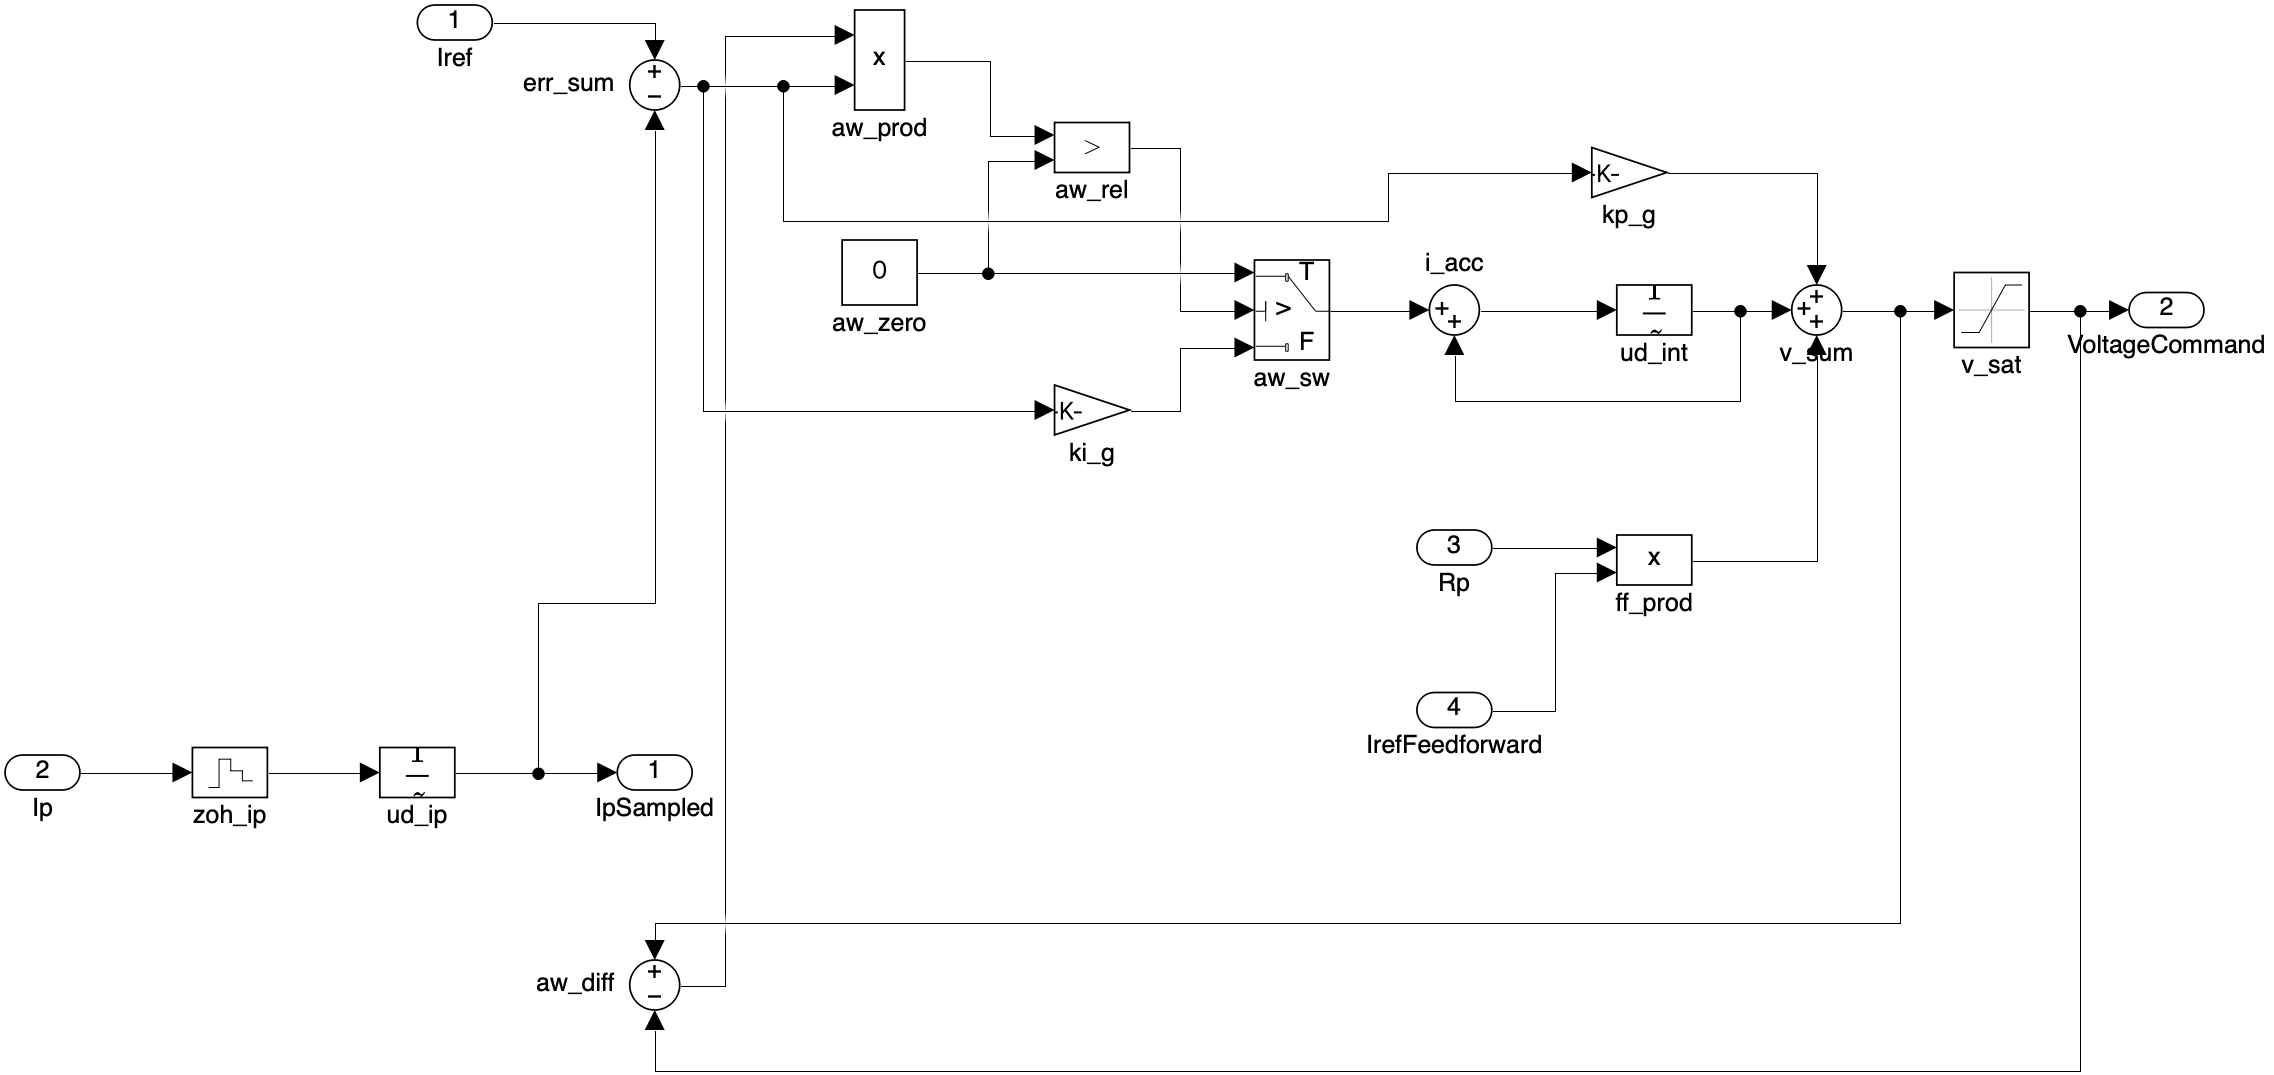
\includegraphics[width=0.56\linewidth]{native/model_current_pi.png}
\caption{\texttt{Current\_PI} 子系统（Simulink 原生视图）：比例积分、抗饱和判据与 $R\sub{p}i\sub{ref}$ 前馈}
\label{fig:pl-pi}
\end{figure}

12.3~s 起切换为退磁控制，被控量改成励磁电流：
\begin{equation}
\hat\psi=L_1(i\sub{cs}-i\sub{p}),\qquad u^{\mathrm{demag}}\sub{AB}=-k_\psi\hat\psi,\quad k_\psi=2\ \mathrm{V/Wb}.
\label{eq:demag}
\end{equation}
纯比例律使磁链按 $1/k_\psi=0.5$~s 的时间常数衰减，输出电压同样限幅 $\pm400$~V。模式切换由受退磁标志控制的 Switch 完成，$i\sub{cs}$ 和 $i\sub{p}$ 先经 50~$\mu$s 采样再进入退磁控制，以避免代数环。

\section{基线模型的运行结果}

实验四的基线模型运行在 2200~V 理想母线上，步长 10~$\mu$s，载波 4~kHz（指导书未重新指定载波频率，基线沿用原设置）。结果见图~\ref{fig:pl-wave} 和表~\ref{tab:pl-plateau}，表中同时列出第 \ref{chap:joint} 章整机模型的同口径结果。

\twofig{native/plasma_startup.pdf}{native/plasma_full_pulse.pdf}{基线模型的 MATLAB 原生波形：(a) 启动段跟踪，(b) 30~s 全过程的电流与功率}{fig:pl-wave}

\begin{dtable}{htbp}{平台段（6--11~s）统计：基线模型与整机模型}
\label{tab:pl-plateau}
\begin{tabularx}{\linewidth}{LRRL}
\toprule
\headrow 物理量 & 基线模型 & 整机模型 & 说明 \\
\midrule
直流母线 & 2200~V & 2199.98~V & 理想源 / 实际母线 \\
载波与步长 & 4~kHz，10~$\mu$s & 2~kHz，1~$\mu$s & 整机含 2~$\mu$s 死区 \\
等离子体电流 $\bar i\sub{p}$ & 10\,006.91~A & 9\,999.28~A & 给定 10~kA \\
线圈电流 $\bar i\sub{cs}$ & 10\,756.87~A & 10\,749.17~A & 含励磁分量约 750~A \\
线圈侧功率 & 1.0879~MW & 1.0781~MW & 桥臂输出 \\
等离子体功率 & 1.0014~MW & 约 1.000~MW & $R\sub{p}i\sub{p}^2$ \\
电流纹波峰峰值 & 304.03~A & 226.55~A & 1.8--1.85~s 窗口 \\
\bottomrule
\end{tabularx}
\end{dtable}

\textbf{启动段。}0.6~s 之前使能为 0、门极封锁；0.6~s 起给定按 10~kA/s 上升，$i\sub{p}$ 几乎无滞后地跟随，1.6~s 到达 10~kA。$u\sub{AB}$ 只需在 0--100~V 之间变化，离限幅很远，整段都是小信号工作。

\textbf{平台段。}$i\sub{cs}$ 由 1.6~s 的约 10.05~kA 爬升到 11.6~s 的约 11.05~kA，增量约 1~kA，正好是励磁电流的增长：磁链以 $R\sub{p}i\sub{p}\approx100$~V 的速率被消耗，$i\sub{m}=\psi/L_1$ 随时间线性增长。线圈侧与等离子体侧的功率差主要是励磁储能的增长率 $i\sub{m}\dd\psi/\dd t\approx750\ \mathrm{A}\times100\ \mathrm{V}=75$~kW，加上 $R\sub{cs}i\sub{cs}^2\approx2.3$~kW 的电阻损耗，合计 77.3~kW。1~$\mu$s 的整机模型实测差值约 78~kW，与之相符；10~$\mu$s 基线为 86.5~kW，偏大的部分与较粗步长下的开关量化有关。

\textbf{降流与退磁。}11.6~s 起给定以 20~kA/s 下降，0.5~s 内跟到零。12.1~s 起 $R\sub{p}$ 在 0.2~s 内升到 100~$\Omega$，12.3~s 切入退磁。开始时 $\hat\psi$ 较大，退磁律输出顶到 $-400$~V，磁链以约 400~Wb/s 的恒定速率下降，$i\sub{cs}$ 由约 1.08~kA 近似线性回落（图~\ref{fig:pl-flux}(a)）。线圈侧在 12.3--30~s 向直流侧净回馈 0.565~MJ。

基线的退磁尾段值得注意：15.5--24~s 内 $i\sub{cs}$ 由 44~A 匀速降到约 9~A，斜率恰为 4~A/s，桥臂输出恒为 $-4.0$~V，对应两只器件的压降。说明此时指令很小，脉宽已低于 10~$\mu$s 步长可分辨的范围，磁链主要靠器件压降衰减。1~$\mu$s 的整机模型没有这一现象，电流按指数收尾，16~s 时已降到 3.9~A。

\twofig{native/plasma_demagnetization.pdf}{native/plasma_flux_crosscheck.pdf}{基线模型的 MATLAB 原生波形：(a) 降流与退磁段的电流和线圈侧功率，(b) 磁链两条路径及其残差}{fig:pl-flux}

\section{数值校核}

磁链的两条路径是这个模型最有价值的校核（图~\ref{fig:pl-flux}(b)）。一条用电流计算，$\psi_i=L_1(i\sub{cs}-k\,i\sub{p})$；另一条用原生 10~$\mu$s 实测电压积分，$\psi_u=\int(v\sub{AB}-R\sub{cs}i\sub{cs})\,\dd t$。全程最大残差约 0.011~Wb，而平台段磁链变化量为 991~Wb。这一比较说明互感参数填写正确、原副边电流方向一致，$L\sub{p}$ 和 $R\sub{p}$ 确实串联在副边回路中，没有被 100~k$\Omega$ 并联支路旁路。

\textbf{电流纹波。}单极性调制下每半个载波周期出现一个电压脉冲，平台段的纹波可以估计为
\begin{equation}
\Delta i\sub{p}\approx\bar u\Bigl(1-\frac{\bar u}{U\sub{dc}}\Bigr)\frac{T_s}{2L_{\sigma,\mathrm{eq}}},
\label{eq:pl-ripple}
\end{equation}
取 $\bar u=100$~V、$L_{\sigma,\mathrm{eq}}=120\ \mu$H，2~kHz 时约为 200~A（2\%），4~kHz 时约为 100~A。表~\ref{tab:pwm} 是同一负载在不同载波和步长下的实测结果，图~\ref{fig:pwm} 是对应的波形。

\begin{dtable}{htbp}{PWM 设置与求解步长对电流纹波的影响（均为 30~s 运行）}
\label{tab:pwm}
\begin{tabularx}{\linewidth}{P{0.46\linewidth}RRR}
\toprule
\headrow 工况 & 平台段 $\bar i\sub{p}$ / A & 纹波峰峰值 / A & 式~\eqref{eq:pl-ripple} 估计 / A \\
\midrule
基线：4~kHz，10~$\mu$s，无死区 & 10\,006.91 & 304.03 & 100 \\
2~kHz，10~$\mu$s，无死区 & 10\,004.37 & 559.55 & 200 \\
2~kHz，1~$\mu$s，原死区实现（2--3~$\mu$s） & 9\,999.19 & 245.47 & 200 \\
整机：2~kHz，1~$\mu$s，修正死区（2~$\mu$s） & 9\,999.28 & 226.55 & 200 \\
\bottomrule
\end{tabularx}
\end{dtable}

平台段脉宽只有约 6--12~$\mu$s，10~$\mu$s 步长会把脉宽量化放大，所以 10~$\mu$s 的纹波明显偏离估计，也不能据此比较载波频率的影响。步长减到 1~$\mu$s 后，实测值接近估计，余下的差异与死区展宽脉冲有关。因此，本报告把 1~$\mu$s 工况的约 2.3\% 作为电流纹波的代表值。

\begin{figure}[htbp]
\centering
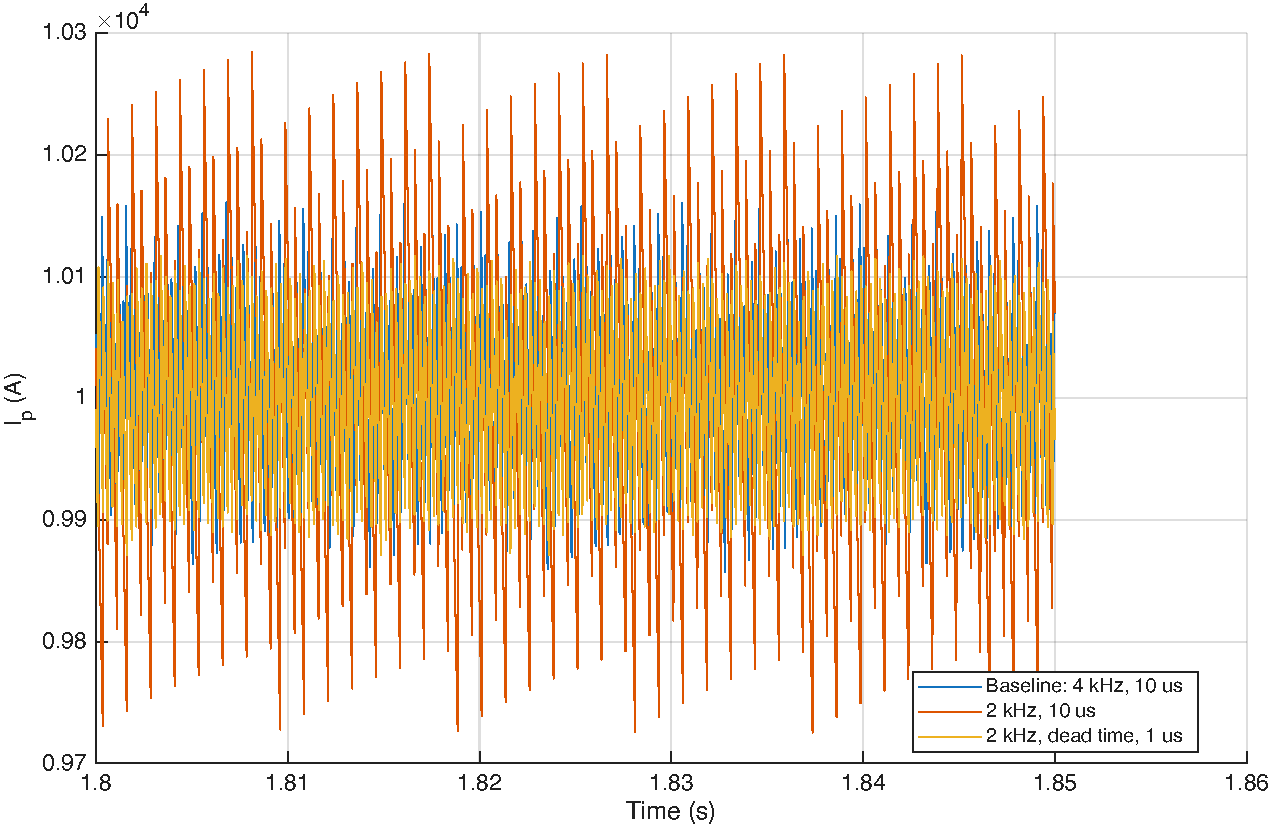
\includegraphics[width=0.5\linewidth]{native/pwm_current_ripple.pdf}
\caption{三种 PWM 设置下 1.8--1.85~s 的电流纹波（MATLAB 原生波形）}
\label{fig:pwm}
\end{figure}
